\chapter{自动驾驶环境算法迁移}
%一个特殊的大实验
\section{自动驾驶实验背景介绍}
自动驾驶成为近年来人工智能领域发展最迅猛的技术之一,Alphabet旗下的子公司Waymo为代表的一批自动驾驶企业已经让车辆上路\cite{waymo}。不过在复杂场景下,这些车辆的行为仍然不够智能,需要人类驾驶员的干预。\par
自Deepmind的科学家在$Nature$发文提出深度强化学习在游戏中的应用后\cite{nature2015},强化学习作为人工智能的下一个发展大方向,也在2015-2018年迎来了爆发点。然而,尽管强化学习在棋牌等游戏中获得了巨大的成功,目前的强化学习在自动驾驶上仍没有成熟的应用。\par
把强化学习应用于自动驾驶是一个极其自然的想法。自动驾驶的应用场景本质上是移动机器人的问题,而强化学习应用于机器人更是由来已久\cite{RL_in_robotics}\cite{Model-Based_RL_robotics}\cite{DRL_for_driving}。因此,在这个项目中我们考虑了一个较为复杂的自动驾驶场景——环岛场景,希望应用强化学习框架,设计出适合于自动驾驶在此类场景中决策的算法。

把强化学习应用于自动驾驶是一个自然的想法,我们可以利用强化学习进行决策,由此构建一个自动驾驶的框架\cite{DRL_for_driving}。\par
在图\ref{fig:self-driving_overview}中,我们绘制了一个框架的示意图。可以看出,决策(decision-making, planning)是自动驾驶的``大脑'',是在不同场景中处理问题的核心算法。\par
      \begin{figure}[h] % use float package if you want it here
        \centering
        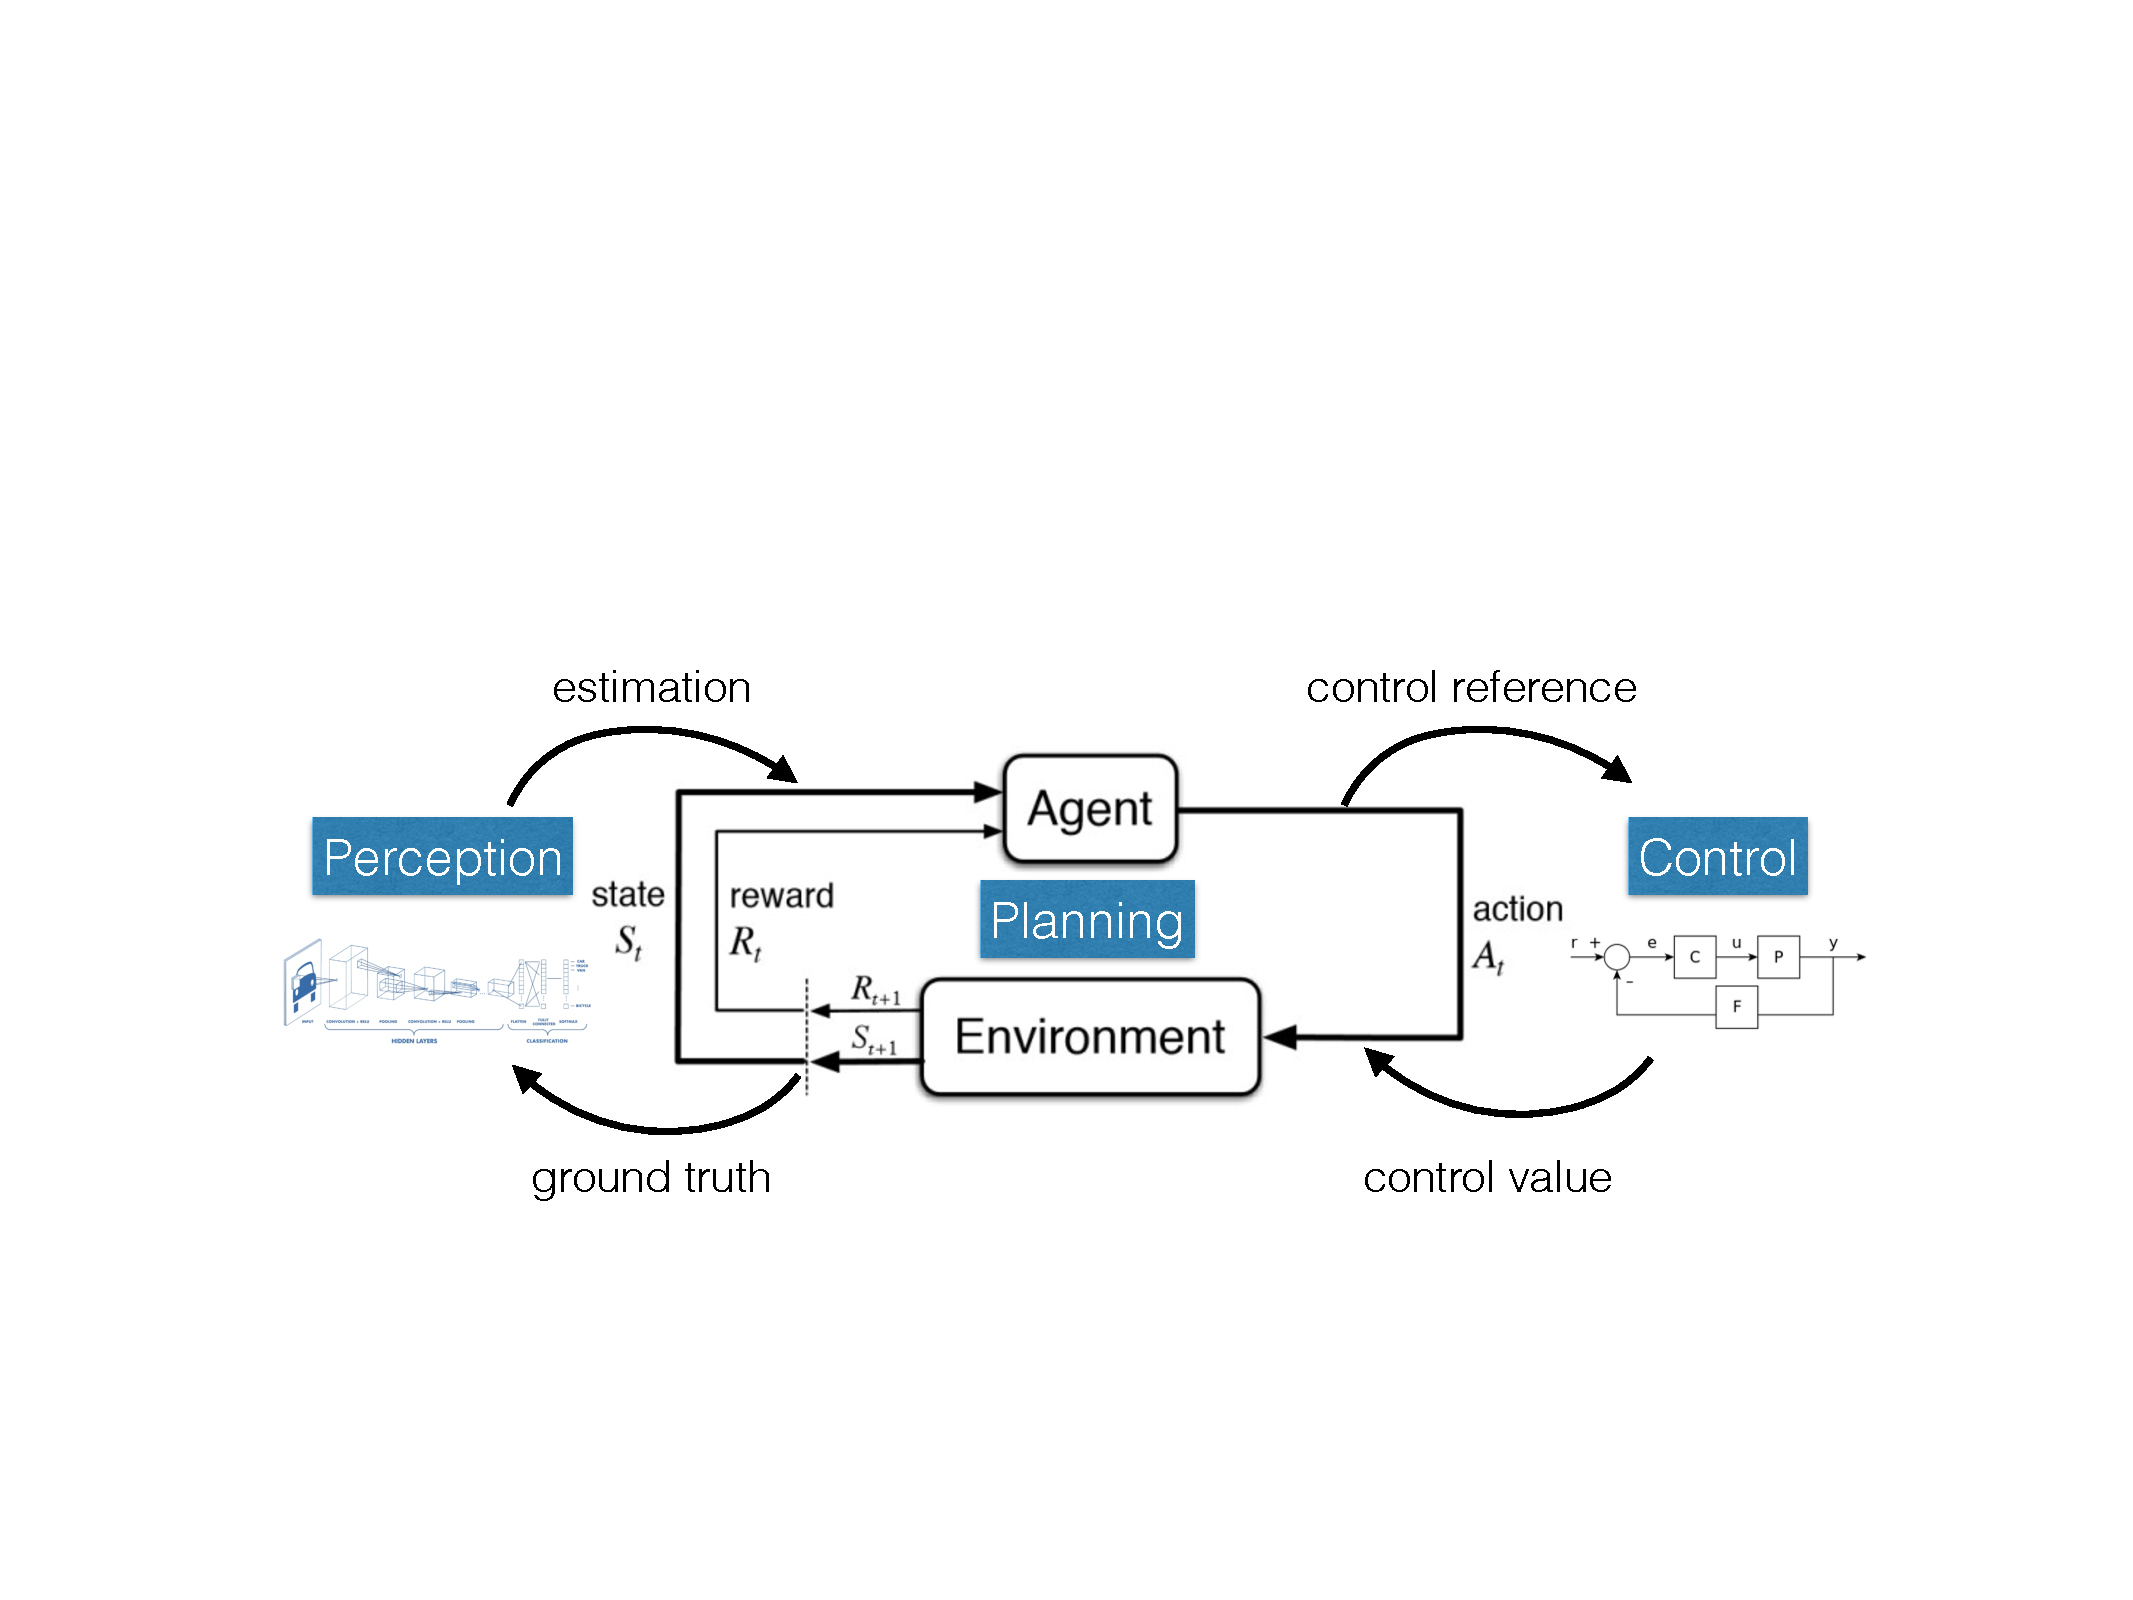
\includegraphics[scale=0.5]{driving_overview}
        \caption{自动驾驶的基本框架:三个回路,从左到右依次是感知,决策,和控制}
        \label{fig:self-driving_overview}
      \end{figure}
事实上,感知算法和控制算法目前都已经做的相应较为成熟,并且由于其一般性更强,因此解决得比较好。相比之下,自动驾驶的决策目前仍然依赖于人工基于规则编码,缺乏泛化的能力。环岛路径规划涉及到与其他智能体的高频交互,例如超车换道,路权退让,环岛路径汇入汇出等,是自动驾驶的一个复杂场景。

  
\section{实验环境}
\subsection{环岛路径规划问题描述}
在本节,我们会对环岛路径规划问题的具体实验设计进行介绍。\par
我们在仿真环境中建设双车道环岛。分为三进口、四进口两类;每一类场景有根据车流密度1辆/5s和1辆/20s(新车进入环岛的频率)分为两种情况,这样一种形成四种实验场景,如示意图\ref{fig:experiments}所示。
      \begin{figure}[H] % use float package if you want it here
        \centering
        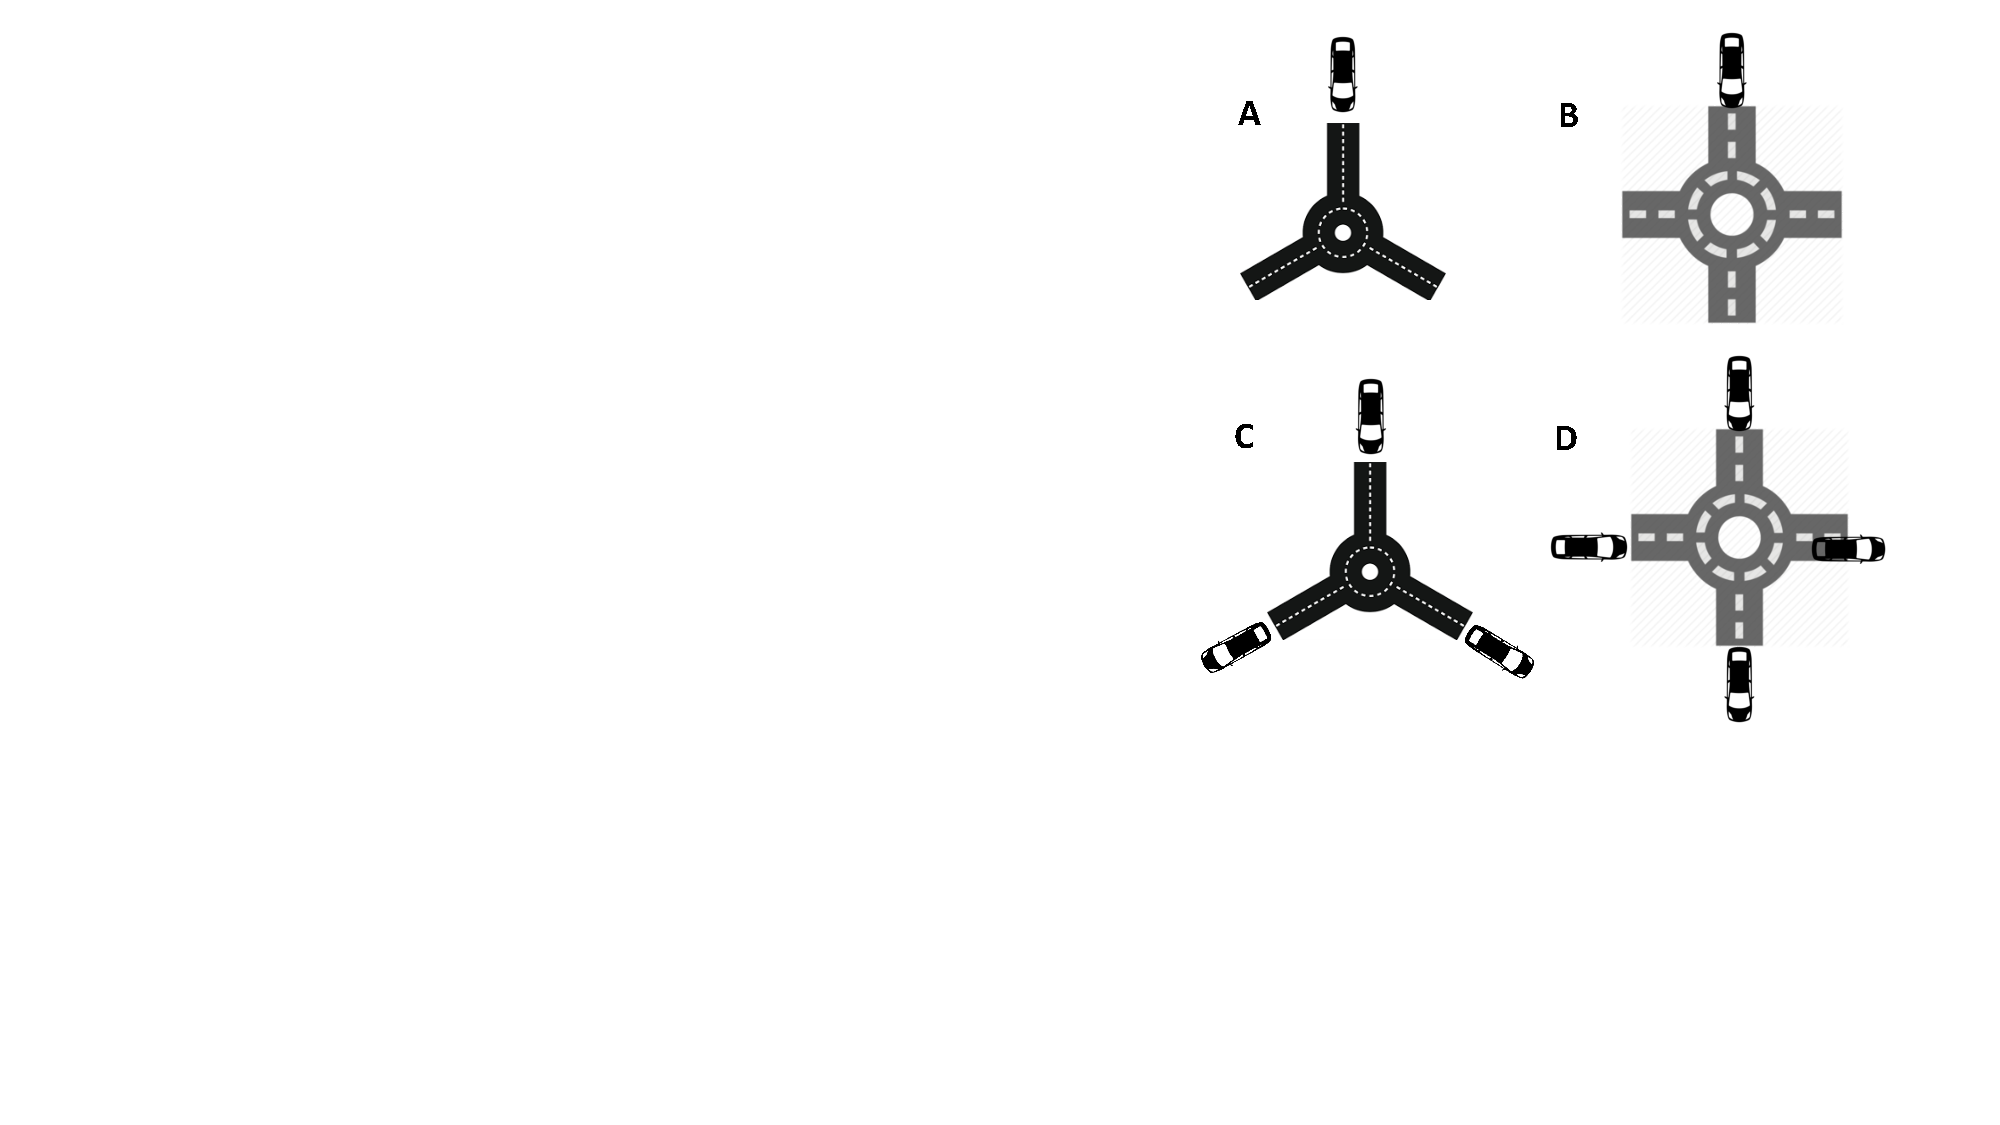
\includegraphics[scale=0.4]{experiments_design}
        \caption{四个实验场景,(A) 三进口,1辆/20s (B) 四进口,1辆/20s (C) 三进口,1辆/5s (D) 四进口,1辆/5s}
        \label{fig:experiments}
      \end{figure}
    \par 所有其他车辆都遵循基于规则的驾驶方案进行驾驶。
    \par 之所以选择四个实验场景,是基于我们对算法的设计。我们将有三套不同的算法在实验环境中进行对比,具体对比内容将在后面介绍。
    \par 具体任务类似于一个最优控制问题。我们对车辆的控制量$u$是一个二维向量,第一维代表刹车/油门强度,第二维表示是否变道。
    $$ u = [u_1\; u_2]^T,\: \space u_1 \in [-1, 1],\: \space u_2 \in {0, 1} $$
    \par 控制目标是让车辆尽快、稳定地无事故地通过环岛。具体如何量化这些指标,取决于我们如何设计强化学习的奖励函数。初始条件是车辆以一个定速度到达环岛入口。和最优控制的区别在于,我们无法用一个简单的微分方程表达车辆的状态方程,因而这个问题也不再是简单的最优控制问题。在理论基础一节,我们会介绍强化学习如何去表达一个复杂环境的动态特性。

\section{环岛实验平台方案}
    实验平台采用SUMO\cite{SUMO}+Webots\cite{Webots}进行搭建。SUMO负责生成交通流,而Webots则用于构建车辆模型。\par
    我们采用强化学习范式来解决环岛路径规划问题。我们把算法研究分为三个阶段。
    \begin{enumerate}
      \item 第I阶段,利用现有算法,解决部分可观测的马尔可夫问题的强化学习。
      \item 第II阶段,结合无模型和基于模型的强化学习算法,用于提升采样效率。
      \item 第III阶段,多任务强化学习框架,具体包括复杂任务分解、相似子任务识别、知识共享、子任务策略重组的方法。
    \end{enumerate}
    \par 这三个阶段的算法将会和之前介绍的四个场景进行结合,从而用于检验算法效果,如表\ref{table:experiments}所示。
    \begin{table}[h!]
    \centering
    \caption{实验设计}
    \label{table:experiments}
    \begin{tabular}[c]{|c|c|c|c|c|}
    \hline
    \textbf{实验场景} & \textbf{I和II对比} & \textbf{I和III对比} & \textbf{II和III对比}\\
    \hline \hline
    A   & 训练时间 & 训练时间 & $\times$ \\ \hline
    B   & 获得奖励值 & 获得奖励值 & 训练时间 \\ \hline
    C   & 获得奖励值 & 获得奖励值 & 训练时间 \\ \hline
    D   & $\times$ & $\times$ & 获得奖励值 \\
    \hline
    \end{tabular}
    \end{table}

\section{基线算法:DDPG}
  \subsection{综述}
  目前已经完成如前所述的算法I的实现和实验。我们利用openAI的baseline算法库\cite{openAI_baselines},采用DDPG\cite{DDPG}算法,结合LSTM\cite{DRQ}搭建网络,在我们的实验平台(SUMO+Webots)上实现了基线方案。\par
  
  \subsection{建模方法}
  简要对我们的我们对观察空间进行这样的建模:我们关注离智能体车辆最近的两辆其他车辆,$C_1$和$C_2$。观察空间定义为
  $$[d^{C_1},\space v^{C_1},\space cos\theta^{C_1},\space sin\theta^{C_1},\space d^{C_2},\space v^{C_2},\space cos\theta^{C_2},\space sin\theta^{C_2},\space
  x^{ego},\space y^{ego},\space v^{ego},\space a^{ego}
  ]^T$$
  其中$d$表示距离,$v$表示速度,$a$表示加速度。\par
  为了避免高维度的动作空间,车辆只决定每一时刻的加速和减速值,介于$[-1, 1]$。车辆的方向由预先规定的路径点决定,由事先设计好的PID控制器直接进行调控,而不受强化学习算法的决策控制。
  
  \subsection{奖励函数设计}
  我们的奖励函数有如下机制:
  \begin{itemize}
    \item $0.95$的奖励,当智能体驶出环岛
    \item $0.2$的奖励,每次足够接近一个预先确定的路径点时
    \item $0.05 \dot (v-19)/30 $,表示速度越快得到的奖励越多
    \item $-0.4$的奖励(惩罚),当智能体偏离道路
    \item $-100$的奖励,当智能体发生碰撞时
  \end{itemize}
  
  \subsection{实验结果}
  实验结果如图\ref{fig:experiment_phaseI}。我们可以看出,汽车在2000次训练后可以以75\%以上的成功率通过环岛。在测试中,我们采用经过500次训练后得到的智能体,在双车道四进口的环岛进行五次测试,环岛车流量分别为1辆/5s和1辆/20s。具体成功率统计数据呈现在表格\ref{table:experiment_phaseI}中。\par
  \begin{figure}[h] % use float package if you want it here
        \centering
        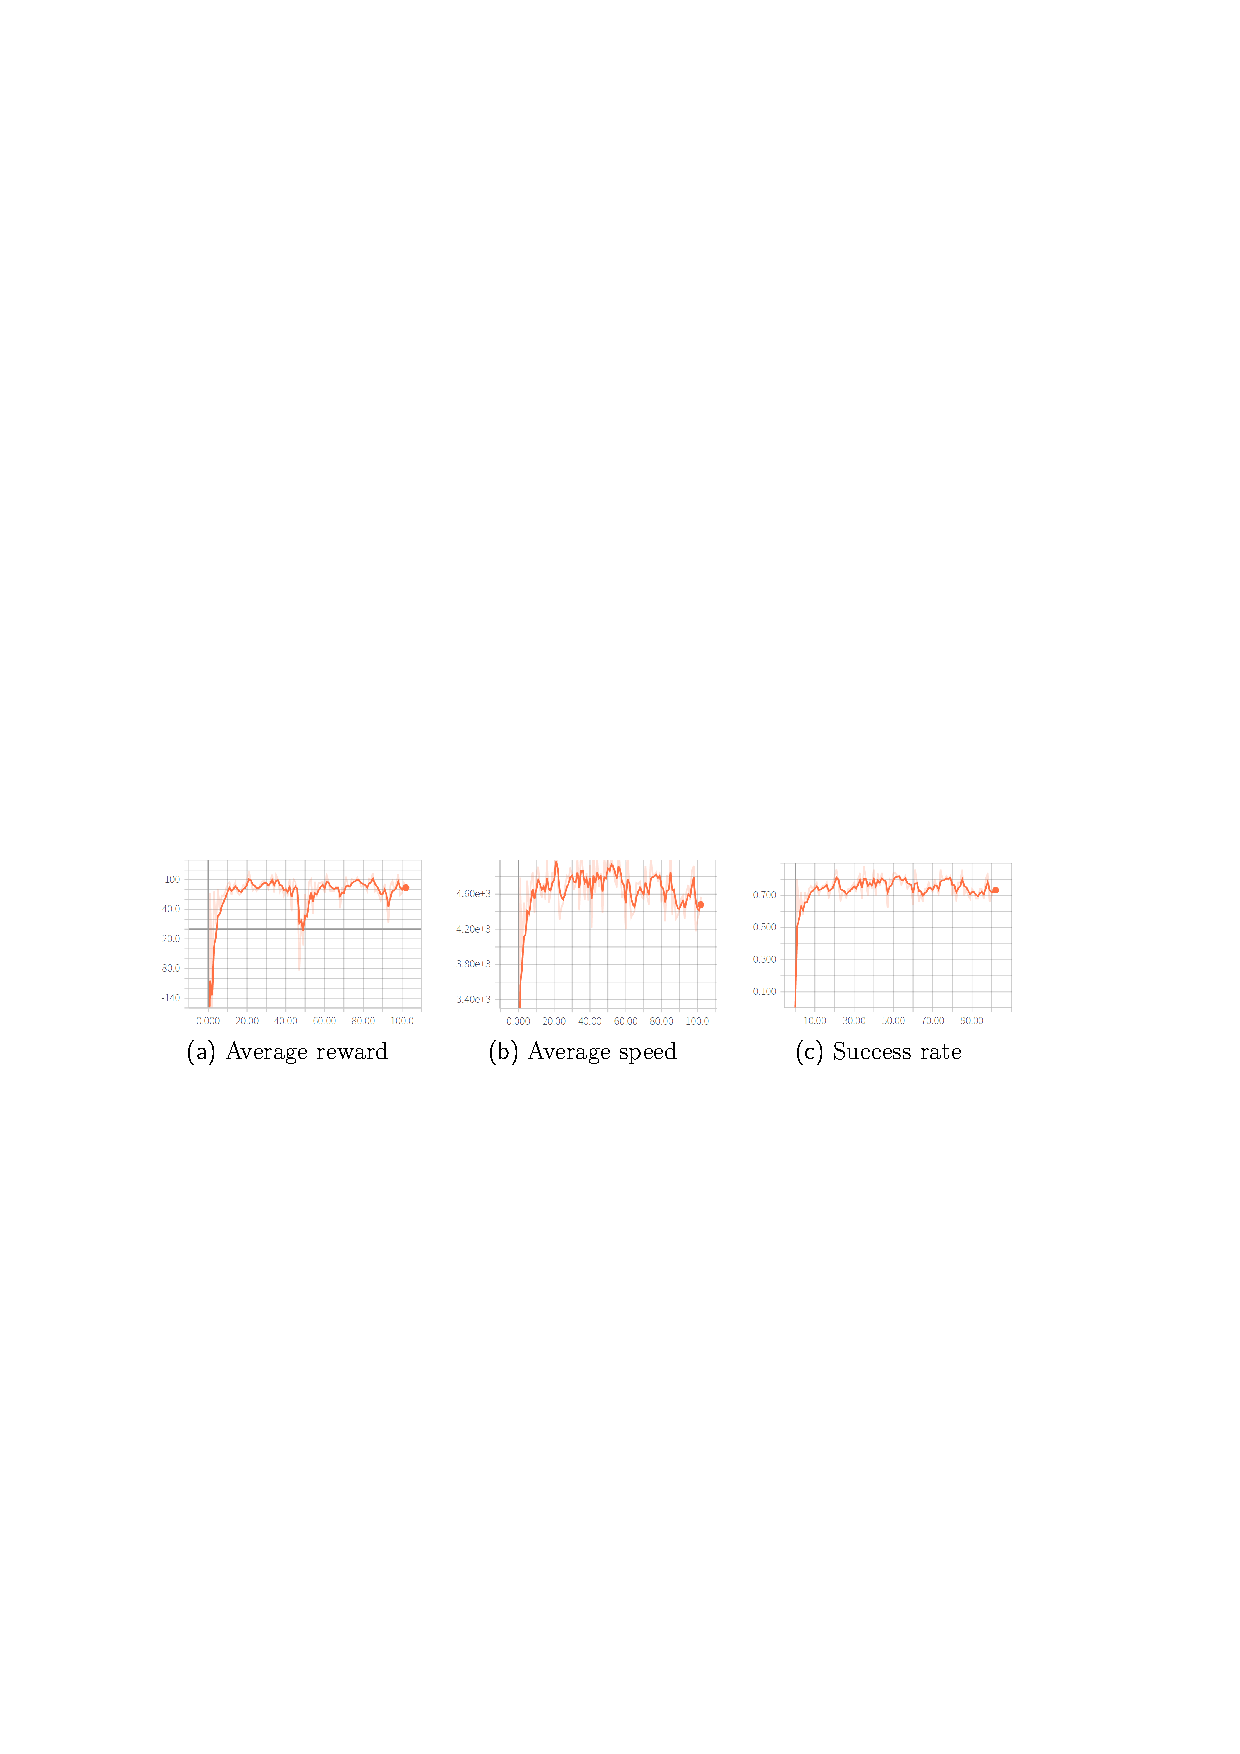
\includegraphics[scale=1.0]{exp_result}
        \caption{DDPG算法训练的实验结果。(a)为平均获得的奖励值(b)为汽车在仿真环境中的平均速度(c)为平均成功率。每个数据点均为五十次训练的平均值,横坐标为百次训练,每次训练以发生事故或通过环岛为终止条件。}
        \label{fig:experiment_phaseI}
  \end{figure}
  
  \begin{table}[h!]
  \centering
  \caption{实验成功率统计(百分比)}
  \label{table:experiment_phaseI}
  \begin{tabular}[c]{|c||c|c|c|c|c||c|}
  \hline
  \textbf{平均车流量$n$(1辆/$n$s)} & \textbf{1}& \textbf{2}& \textbf{3}& \textbf{4}& \textbf{5}& \textbf{平均成功率}\\
  \hline
  5 & 75.4 & 73.8 & 75.0 & 77.0 & 74.8 & 75.2 $\pm$ 1.0 \\ \hline
  20 & 94.0 & 94.4 & 94.0 & 94.6 & 97.0 & 94.8 $\pm$ 1.1 \\ \hline
  \end{tabular}
  \end{table}
  
\section{HAAR应用于环岛路径规划}
\subsection{底层技能预训练}
在本节中,我们把HAAR算法应用于环岛路径规划的场景进行实验。首先我们需要划分什么是自动驾驶车辆的``技能''。我们把环岛依据其地形特点分为几个不同的部分,如图\ref{fig:train_self_driving}所示。通过设定起点和终点,我们训练自动驾驶车辆在各段道路内完成任务,可以由此人为地得到几个子技能。

      \begin{figure}[h] % use float package if you want it here
        \centering
        \includegraphics[scale=0.6]{train_self_driving}
        \caption{按照路线特征划分为四个阶段,分别预训练。}
        \label{fig:train_self_driving}
      \end{figure}

\subsection{上下层策略共同训练}
在获得底层技能以后,我们再训练上层策略根据环境输入挑选底层策略。基本思路和前文提到的HAAR算法相同。受时间限制,此部分工作将在今后进一步完善。

\section{自动驾驶实验总结}
我们设计了一个具有较高复杂性的自动驾驶环岛路径规划问题。通过简化模型,我们让自动驾驶车辆沿一定的轨迹运行,希望它能够识别自己所处的不同状态,采取相应的策略。利用传统的强化学习算法,我们在低流量的情况下已经实现了较高的成功率。但是在高流量的情况下,传统算法仍然难以做到避免碰撞。为此,我们希望利用HAAR算法的分层结构来提高训练的效率。

注意到,HAAR本来是设计给稀疏奖励问题的。如果环境的流量非常高,而我们给车辆设计一些特殊的奖励函数,那么这个问题就已经不再是稀疏奖励问题。因此,HAAR本身是否能够在这个特定问题中起到充分的作用,是未必可以保证的(参考在蚂蚁食物收集环境中的训练结果)。但是,分层结构本身将会大大提高训练的采样效率,从而加速训练。因此,在后续的实验中,我们会把采样效率作为一个重要指标进行考虑。此部分工作仍在进行中,因此结论也有待进一步的研究分析。


